\chapter{Estudio de viabilidad}
    Para poder dar inicio a este proyecto es necesario evaluar previamente sus posibilidades reales de éxito. Esta etapa no se centra solo en su desarrollo inicial como TFG, sino enfocado también a una potencial evolución futura más allá del ámbito académico.

   Con el objetivo de saber si realmente merece la pena invertir esfuerzos y recursos en esta aplicación, hay que examinar el proyecto desde distintas perspectivas, identificando tanto los factores que juegan a favor como aquellos obstáculos que podrían dificultar su progreso o limitar su impacto.

   Hay que tener en cuenta que este proyecto no se trata de inventar algo completamente nuevo. Ya existen herramientas en el mercado que abordan parcialmente problemas similares, pero en este caso está el propósito de mejorar esas propuestas actuales y adaptarse mejor a las necesidades específicas de los profesionales del sector.

   A continuación, se aplicarán distintas metodologías de análisis que permitirán obtener una visión completa de la situación. De esta forma, se podrá determinar la solidez del proyecto.

  
\section{Análisis DAFO} 

    El análisis DAFO (Debilidades, Amenazas, Fortalezas y Oportunidades), también conocido por sus siglas en inglés como análisis SWOT (Strengths, Weaknesses, Opportunities, Threaths), es una herramienta de diagnóstico ampliamente utilizada en la gestión de proyectos y la planificación empresarial\footnote{\cite{weihrich1982daws}}. Sirve para evaluar la situación actual de un producto o servicio, identificando tanto los factores internos como externos que pueden influir en su desarrollo y éxito.

    Esta metodología tiene 4 dimensiones principales, al ser una matriz 2x2. La primera examina los factores internos del proyecto, sobre los que se tiene control directo, clasificándolos como fortalezas (ventajas competitivas) y debilidades (limitaciones o carencias). Por otro lado, se analizan los factores externos, sobre los que no se ejerce control pero que afectan al proyecto, siendo oportunidades (circunstacias favorables aprovechables) y amenazas (riesgos que pueden comprometer el progreso).

    El principal objetivo de este análisis es proporcionar una visión para tomar decisiones que potencien las fortalezas, mitiguen las debilidades, exploten las oportunidades y anticipen las amenazas. Dado que en este proyecto académico convergen distintos factores técnicos, económicos y sociales, resulta conveniente.
\begin{itemize}
\item \textbf{Fortalezas}: Una fortaleza destacable es la actualidad y relevancia del problema que se pretende resolver. Las tecnologías inmersivas tienen cada vez más presencia en el día a día, abriendo muchas posibilidades de innovación en el futuro. Por otro lado, la industria de la construcción es imprescindible e indispensable para la práctica totalidad de las civilizaciones, por lo que es un proyecto muy versátil para muchas empresas.

En segundo lugar, este proyecto es desarrollado por una persona, lo que optimiza la toma de decisiones, ya que, a excepción del tutor, no se necesita mucha más validación. Además, no requiere coordinar el progreso de este proyecto con otras personas. Los objetivos serán más claros ya que el producto tendrá el límite de capacidad de trabajo de una sola persona, centrándose en desarrollar los aspectos más imprescindibles.

Por último, el autor ya tiene experiencia en el uso de dispositivos de realidad virtual/aumentada, aunque sin tener conocimientos de todas las posibilidades que tiene, ya está familiarizado con las interfaces, controles y funciones básicas de éstos.

\item \textbf{Debilidades}: A pesar de tener experiencia en el uso práctico de estas tecnologías, una de las debilidades más destacables es la falta de conocimiento en el campo de desarrollo específicamente, como se ha comentado en la motivación, uno de los objetivos de este TFG es introducirse en la industria de aplicaciones AR/VR y ver si es algo en lo que especializarse, por lo que aspectos como el seguimiento espacial, optimización para renderizado en tiempo real y diseño de interfaces tridimensionales difieren del desarrollo software convencional, lo que implica invertir más tiempo para familiarizarse con nuevas tecnologías de desarrollo.

Otra debilidad es la falta de recursos financieros. Aunque existen a disposición herramientas de desarrollo gratuitas o con licencias educativas, ciertos aspectos como acceder a librerías premium o assets podría requerir inversión económica. Esta limitación condiciona las decisiones tecnológicas y puede afectar al alcance funcional del producto final.

Después estarían las obligaciones académicas simultáneas, al estar cursando el último año de Ingeniería Multimedia a tiempo completo, esto restará tiempo que se podría invertir en este proyecto, ralentizando el progreso y dificultando el mantener la concentración en aspectos complejos del proyecto.

Finalmente, la limitación de alcance inherente a un TFG impide desarrollar un producto completamente funcional y comercializable. El tiempo disponible obligará a priorizar funcionalidades imprescindibles y a implementar prototipos o demostraciones de concepto en lugar de sistemas robustos listos para producción y venta, afectando la viabilidad real de esta aplicación.

\item \textbf{Oportunidades}: Este proyecto presenta un contexto actual que da múltiples oportunidades favorables para su aplicación práctica. La creciente adopción de metodologías BIM en el sector de la construcción, impulsada incluso por normativas en diversos países\footnote{~\cite{ukcabinet2016strategy, eubim2017handbook, fomento2015comision}}, genera una base de datos de modelos 3D estructurados que pueden servir como información para alimentar la aplicación.

Por otro lado, la evolución acelerada de dispositivos AR/VR representa otra oportunidad considerable. Los smartphones actuales incorporan capacidades AR nativas, las gafas de realidad mixta están mejorando rápidamente, y las plataformas VR son cada vez más accesibles. Esto amplía el público potencial que podría beneficiarse de la solución.

La disponibilidad de comunidades online especializadas en desarrollo AR/VR, foros técnicos, tutoriales y documentación abierta facilita enormemente el aprendizaje autodidacta y la resolución de problemas técnicos. Plataformas como Github o Meta For Developers constituyen herramientas casi imprescindibles para el desarrollo.

\item \textbf{Amenazas}: La competencia establecida quizá suponga la amenaza más evidente, empresas especializadas con años de experiencia, equipos multidisciplinares y recursos financieros sustanciales ya ofrecen soluciones AR/VR. Aunque sea a nivel conceptual, competir con dichas entidades podría suponer un obstáculo importante.

Los rápidos cambios tecnológicos en la industria AR/VR representan otra amenaza. Frameworks, \gls{sdks} y dispositivos evolucionan constantemente, lo que podría desembocar a decisiones obsoletas tomadas al inicio del proyecto antes de su finalización. Además, el dispositivo de uso personal del desarrollador no es el modelo más reciente, por lo que podría tener limitaciones de recursos o funcionalidades, incluso es posible que descontinuen dispositivos o modifiquen \gls{apis}, lo que obligaría a adaptar el desarrollo sobre la marcha.

Además, en un contexto práctico para la aplicación, vulnerabilidades de seguridad y privacidad inherentes a aplicaciones que capturan información espacial del entorno real y gestionan datos sensibles de proyectos constructivos presentan riesgos significativos. Podría comprometer datos confidenciales de clientes o generar responsabilidades legales, especialmente en un contexto donde la normativa sobre protección de datos (\gls{gdpr} en Europa) es cada vez más estricta\footnote{\cite{eu2016gdpr}}.
\end{itemize}

\begin{table}[!htb]
\centering
\caption{Matriz DAFO del proyecto}
\label{tab:dafo}
\begin{tabular}{|p{4cm}|p{4cm}|}
\hline
\textbf{Fortalezas} & \textbf{Oportunidades} \\
\hline
Relevancia del problema. & Creciente adopción de metodologías BIM. \\
Experiencia práctica previa. & Disponibilidad de guías online. \\
\hline
\textbf{Debilidades} & \textbf{Amenazas} \\
\hline
Curva de aprendizaje en realidad extendida. & Rápida evolución de los frameworks de Oculus. \\
Limitaciones de hardware. & Posible aparición de soluciones similares. \\
\hline
\end{tabular}
\end{table}

\section{Lean Canvas} 

El Lean Canvas (Cuadro~\ref{tab:lean-canvas})  es una herramienta de modelado empresarial derivada del Business Model Canvas, pero está adaptada para startups y proyectos en fase inicial como este. Es especialmente útil cuando existen muchas incertidumbres sobre el producto o servicio que se pretende desarrollar. Además, da una visión sobre cómo podría evolucionar esta solución en un entorno real si se decidiera continuar su desarrollo tras finalizar los estudios\footnote{\cite{maurya2012running}}.

Consiste en nueve bloques que permiten visualizar brevemente los aspectos fundamentales del modelo de negocio, es decir, a quién va dirigido, qué problema resuelve, cómo lo resuelve, cómo llegará a sus usuarios y cómo generará valor, tanto para los clientes como para el proyecto mismo. Lean Canvas consiste en un marco estructurado para organizar ideas, detectar inconsistencias y comunicar la propuesta de valor de forma clara. Sin embargo, no es una investigación de mercado minuciosa ni proporciona datos cuantitativos precisos sobre tamaño de mercado.

- \textbf{Segmentos de cliente}: El público objetivo de esta aplicación está principalmente dirigido a los profesionales de la construcción.
\begin{itemize}
\item Estudios de arquitectura e ingeniería: Especialmente los que trabajan con metodologías BIM y buscan formas innovadoras de presentar sus proyectos a cliente o validar decisiones de diseño internamente.
\item Empresas constructoras y contratistas: Profesionales que necesitan herramientas para inspeccionar obras, detectar discrepancias entre proyecto y ejecución, y coordinar equipos multidisciplinares en campo.
\item Promotoras inmobiliarias: Compañías interesadas en ofrecer experiencias inmersivas a potenciales compradores antes de que el edificio esté construido.
\item Responsables de obra y project managers: Figuras que coordinan múltiples agentes y requieren visualizar el estado del proyecto de forma comprensible para facilitar la toma de decisiones y la comunicación con stakeholders no técnicos.
\item Centros de formación y universidades: Instituciones que imparten grados o másteres en arquitectura, ingeniería civil o construcción, y que podrían utilizar la aplicación como herramienta pedagógica para enseñar procedimientos de seguridad, fases constructivas o interpretación de modelos BIM.
\end{itemize}
- \textbf{Problema}:
\begin{itemize}
\item Dificultad para comunicar proyectos arquitectónicos a clientes o inversores que carecen de formación técnica y no logran interpretar correctamente planos 2D o comprender el espacio real a partir de renders estáticos.
\item Errores constructivos no detectados a tiempo: Discrepancias entre el diseño BIM y la ejecución física que solo se identifican cuando ya se han materializado, generando sobrecostes y retrasos significativos.
\item Falta de herramientas intuitivas para inspección de obra: Los profesionales deben contrastar continuamente documentación en papel o tablets con lo construido, un proceso tedioso y propenso a errores de interpretación.
\item Barreras en la colaboración multidisciplinar: Arquitectos, ingenieros, contratistas y clientes manejan información fragmentada en distintos formatos, lo que dificulta mantener una visión compartida del proyecto.
\item Limitaciones de las herramientas actuales: Las soluciones AR/VR existentes suelen ser caras, estar diseñadas para casos de uso muy específicos, presentar curvas de aprendizaje pronunciadas o no integrarse adecuadamente con los flujos de trabajo BIM establecidos.
\end{itemize}
- \textbf{Propuesta de valor única}: Visualizar y validar tu proyecto constructivo de manera virtual o en el lugar de la obra antes y/o después de construir.

Esta aplicación integra AR y/o VR para permitir que cualquier profesional de la construcción pueda superponer el modelo BIM sobre el emplazamiento real mediante sus gafas de realidad extendida, o explorarlo inmersivamente en VR desde cualquier ubicación. Todo ello sin necesidad de ser experto en tecnología y con integración directa desde los modelos BIM que ya utilizan diariamente. A diferencia de soluciones fragmentadas que solo cubren presentaciones a clientes o solo inspecciones, esta propuesta abarca todo el ciclo de proyecto con una única plataforma accesible y específicamente diseñada para las necesidades del sector de la construcción.

- \textbf{Solución}: Se materializa en:
\begin{itemize}
\item Aplicación VR para gafas de realidad virtual que permite recorrer virtualmente el proyecto completo, evaluar alternativas de diseño y realizar formaciones inmersivas en procedimientos de seguridad.
\item Sistema de importación y optimización BIM que procesa archivo en formatos estándar (\gls{ifc} y Revit) y los convierte automáticamente en modelos optimizados para renderizado en tiempo real.
\item Funcionalidades de anotación y reporte: Los usuarios pueden marcar discrepancias detectadas directamente sobre el modelo AR/VR, adjuntar fotografías, comentarios y generar informes estructurados que se sincronizan con el equipo.
\item Modo colaborativo: Múltiples usuarios pueden visualizar y comentar simultáneamente el mismo proyecto, facilitando reuniones de coordinación donde  todos comparten la misma perspectiva visual.
\end{itemize}
La arquitectura técnica se basa en frameworks consolidados como Unity o Unreal y librerías (ARCore/ARKit), garantizando escalabilidad y mantenibilidad.

- \textbf{Canales de difusión}:
\begin{itemize}
\item Ferias y congresos del sector construcción: Participación en eventos especializados (ej. BIM International Conference\footnote{\cite{eubim}}, Smart City Expo\footnote{\cite{smartcityexpo}}) con demostraciones en vivo que permitan a profesionales experimentar directamente las capacidades de la solución.
\item Colaboraciones con fabricantes BIM: Establecer partnerships con empresas como Autodesk (Revit), Graphisoft (ArchiCAD) o Trimble (SketchUp) para integrar la aplicación en sus plataformas y aparecer en sus marketplaces.
\item Marketing digital especializado: Campañas en LinkedIn dirigidas específicamente a perfiles profesionales del sector (arquitectos y project managers), contenido técnico en blogs especializados y tutoriales en YouTube demostrando casos de uso reales.
\item Prescripción universitaria: Acuerdos con universidades que imparten grados de arquitectura o ingeniería para ofrecer licencias educativas, creando una base de usuarios futuros profesionales familiarizados con la herramienta.
\item Boca a boca y casos de éxito: Publicación de estudios de caso con métricas concretas sobre ahorro de tiempo o reducción de errores en proyectos reales, incentivando la recomendación entre profesionales.
\end{itemize}
- \textbf{Flujos de ingreso}:
\begin{itemize}
\item Suscripción por niveles: Plan básico gratuito con funcionalidades limitadas (visualización de modelos pequeños, sin colaboración), plan profesional (15-30€/mes por usuario) con todas las funcionalidades AR/VR y almacenamiento ampliado, y plan empresarial (precio personalizado) con soporte técnico dedicado, integraciones personalizadas y despliegue on-premise si se requiere.
\item Licencias educativas: Tarifas reducidas para instituciones académicas que deseen utilizar la aplicación como herramienta docente, generando ingresos recurrentes y construyendo base de usuarios futuros.
\item Servicios profesionales: Consultoría para implementación en flujos de trabajo específicos de grandes constructoras, formación personalizada a equipos y desarrollo de funcionalidades a medida bajo contrato.
\item Marketplace de contenidos: Comisión sobre ventas de plantillas, bibliotecas de materiales optimizados para AR/VR o extensiones desarrolladas por terceros que amplíen las capacidades base de la aplicación.
\end{itemize}
- \textbf{Estructura de costes}:
\begin{itemize}
\item Desarrollo software: Aunque inicialmente asumido como proyecto de TFG, un desarrollo completo requeriría contratar o externalizar programadores especializados en Unity/Unreal, desarrolladores móviles y expertos en optimización 3D. Coste estimado: 50.000-80.000€ para \gls{mvp} funcional.
\item Licencias software: Unity Pro o Unreal Engine (aunque gratuitos hasta ciertos umbrales de ingresos), licencias de middleware para procesamiento BIM, herramientas de desarrollo y testing. Coste estimado: 3.000-5.000€/año.

\begin{figure}[!htb]
    \centering
    % ---- PRIMERA IMAGEN ----
    \begin{minipage}[b]{0.48\linewidth}
        \centering
        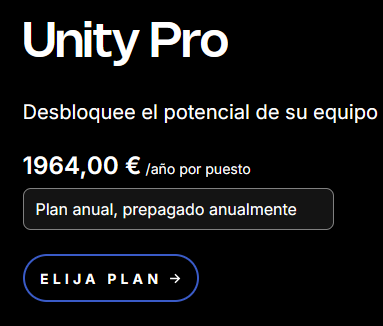
\includegraphics[width=\linewidth]{include/images/unitypro.png}
        \caption{Precio anual de Unity Pro}
        \label{fig:unitypro}
    \end{minipage}
    \hfill
    % ---- SEGUNDA IMAGEN ----
    \begin{minipage}[b]{0.48\linewidth}
        \centering
        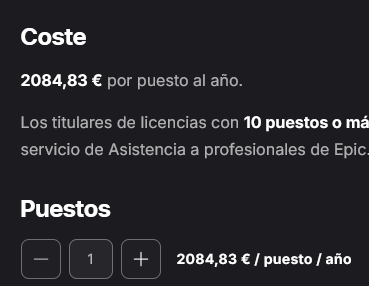
\includegraphics[width=\linewidth]{include/images/unrealenginepro.PNG}
        \caption{Precio anual de Unreal Engine}
        \label{fig:unrealenginepro}
    \end{minipage}
\end{figure}





\item Hardware para testing: Dispositivos móviles de diferentes gamas, gafas AR (HoloLens, Magic Leap) y VR (Quest, Vive) para pruebas exhaustivas. Inversión inicial: 10.000-15.000€.
\item Marketing y ventas: Campañas publicitarias, participación en ferias, material promocional, equipo comercial. Coste variable: 10.000-30.000€/año inicialmente.
\item Legal y administrativo: Registro de empresa, asesoría legal para contratos, cumplimiento GDPR, seguros profesionales. Coste estimado: 5.000-8.000€/año.
\end{itemize}
- \textbf{Métricas claves}: Para evaluar el éxito y evolución del proyecto, se monitorizarán las siguientes métricas:
\begin{itemize}
\item Usuarios activos mensuales: Número de profesionales que utilizan efectivamente la aplicación al menos una vez al mes, diferenciando entre usuarios gratuitos y de pago.
\item Tasa de conversión freemium-premium: Porcentaje de usuarios que migran del plan gratuito a suscripciones de pago, indicador fundamental de la percepción de valor añadido.
\item Tiempo medio de uso por sesión: Métrica que refleja el "compromiso" real con la aplicación; sesiones muy cortas podrían indicar problemas de usabilidad o falta de utilidad percibida.
\item \gls{nps}: Índice de satisfacción que mide la probabilidad de que los usuarios recomienden la aplicación a amigos, crucial en un mercado \gls{b2b} donde la prescripción profesional es determinante.
\item Reducción de errores constructivos detectados: Métrica cualitativa obtenida mediante encuestas a usuarios, que cuantifica el impacto real en la eficiencia de los proyectos.
\item \gls{cac} vs \gls{ltv}: Ratio que determina la sostenibilidad económica del modelo, indicando si el coste de adquisición de cada cliente es inferior al valor que aporta durante su ciclo de vida.
\item Tasa de retención mensual: Porcentaje de usuarios que continúan utilizando la aplicación mes a mes, indicador de la solidez del producto y la fidelización conseguida.
\end{itemize}
- \textbf{Ventaja diferencial}: Los elementos que diferencian esta propuesta de las soluciones competidoras existentes son:
\begin{itemize}
\item A diferencia de herramientas especializadas solo en presentación a clientes o solo en inspección de obra, esta aplicación cubre todas las fases desde el diseño inicial hasta la ejecución final con una única plataforma coherente.
\item Accesibilidad tecnológica: Funciona con gafas convencionales para AR (no requiere equipamiento caro como HoloLens) y ofrece experiencias VR en gafas de gama media, democratizando el acceso frente a soluciones enterprise de alto coste.
\item Experiencia de usuario simplificada: Curva de aprendizaje mínima mediante interfaces intuitivas diseñadas para profesionales no técnicos, eliminando la barrera de entrada que presentan herramientas complejas que requieren formación extensiva.
\end{itemize}

\begin{table}[!htb]
\centering
\caption{Lean Canvas del proyecto}
\label{tab:lean-canvas}
\resizebox{\textwidth}{!}{
\footnotesize
\begin{tabular}{|>{\raggedright\arraybackslash\hspace{0pt}}p{2.8cm}|>{\raggedright\arraybackslash\hspace{0pt}}p{2.8cm}|>{\raggedright\arraybackslash\hspace{0pt}}p{2.8cm}|>{\raggedright\arraybackslash\hspace{0pt}}p{2.8cm}|>{\raggedright\arraybackslash\hspace{0pt}}p{2.8cm}|}
\hline
\textbf{PROBLEMA} & \textbf{SOLUCIÓN} & \textbf{PROPUESTA DE VALOR ÚNICA} & \textbf{VENTAJA DIFERENCIAL} & \textbf{SEGMENTOS DE CLIENTE} \\
\hline
\begin{itemize}[leftmargin=*,noitemsep,topsep=2pt,itemsep=4pt]
    \item Dificultad para comunicar proyectos a clientes no técnicos
    \item Errores constructivos no detectados a tiempo
    \item Falta de herramientas intuitivas para inspección
    \item Barreras en colaboración multidisciplinar
    \item Limitaciones de herramientas actuales
\end{itemize}
&
\begin{itemize}[leftmargin=*,noitemsep,topsep=2pt,itemsep=4pt]
    \item App VR para gafas de realidad virtual
    \item Sistema de importación BIM (IFC, Revit)
    \item Anotación y reporte
    \item Modo colaborativo
\end{itemize}
&
\begin{itemize}[leftmargin=*,noitemsep,topsep=2pt,itemsep=4pt]
    \item Integración AR/VR accesible sin ser experto.
\end{itemize}
&
\begin{itemize}[leftmargin=*,noitemsep,topsep=2pt,itemsep=4pt]
    \item Integración completa AR y/o VR
    \item Interoperabilidad BIM real
    \item Experiencia de usuario simplificada
\end{itemize}
&
\begin{itemize}[leftmargin=*,noitemsep,topsep=2pt,itemsep=4pt]
    \item Estudios de arquitectura e ingeniería
    \item Empresas constructoras
    \item Promotoras inmobiliarias
    \item Project managers
    \item Centros formativos
\end{itemize}
\\
\hline
& \textbf{MÉTRICAS CLAVE} & & \textbf{CANALES} & \\
\cline{2-2} \cline{4-4}
&
\begin{itemize}[leftmargin=*,noitemsep,topsep=2pt,itemsep=3pt]
    \item Usuarios activos mensuales (MAU)
    \item Conversión freemium/premium
    \item Tiempo uso por sesión
    \item Net Promoter Score
    \item Reducción errores detectados
    \item CAC vs LTV
    \item Retención mensual
\end{itemize}
& &
\begin{itemize}[leftmargin=*,noitemsep,topsep=2pt,itemsep=3pt]
    \item Ferias y congresos sector
    \item Colaboración fabricantes BIM
    \item Marketing digital (LinkedIn)
    \item Prescripción universitaria
    \item Casos de éxito
\end{itemize}
& \\
\hline
\multicolumn{3}{|c|}{%
    \begin{minipage}[t]{\dimexpr 8.4cm + 4\tabcolsep + 2\arrayrulewidth\relax}
        \vspace{0.15cm}
        \textbf{ESTRUCTURA DE COSTES} \par \vspace{0.1cm}
        \begin{itemize}[leftmargin=*,noitemsep,topsep=0pt,itemsep=3pt]
            \item Desarrollo software (50.000-80.000€ MVP)
            \item Licencias software (3.000-5.000€/año)
            \item Hardware testing (10.000-15.000€)
            \item Marketing (10.000-30.000€/año)
            \item Legal y administrativo (5.000-8.000€/año)
        \end{itemize}
        \vspace{0.15cm}
    \end{minipage}%
} & 
\multicolumn{2}{c|}{%
    \begin{minipage}[t]{\dimexpr 5.6cm + 2\tabcolsep + \arrayrulewidth\relax}
        \vspace{0.15cm}
        \textbf{FLUJOS DE INGRESOS} \par \vspace{0.1cm}
        \begin{itemize}[leftmargin=*,noitemsep,topsep=0pt,itemsep=3pt]
            \item Suscripción freemium: básico gratuito, profesional 15-30€/mes, empresarial personalizado
            \item Licencias educativas
            \item Servicios profesionales (consultoría, formación)
            \item Marketplace de contenidos
        \end{itemize}
        \vspace{0.15cm}
    \end{minipage}%
} \\
\hline
\end{tabular}
}
\end{table}


\section{Análisis de riesgos} 

El análisis de riesgos, visto en el Cuadro~\ref{tab:riesgos} permite identificar anticipadamente aquellos eventos o circunstancias que podrían impactar negativamente en el desarrollo del proyecto, evaluando su probabilidad de ocurrencia y su potencial impacto\footnote{\cite{pmi2017pmbok}}. A diferencia del análisis DAFO que examina amenazas externas de forma general, este apartado se centra en riesgos concretos con estrategias específicas de mitigación. Esta herramienta permitirá aumentar significativamente las probabilidades de éxito del proyecto, anticipando problemas antes de que se materialicen y estableciendo planes de contingencia para aquellos que, inevitablemente, surgirán durante el desarrollo.

- \textbf{Riesgos técnicos}:
\begin{itemize}
\item Rendimiento insuficiente en dispositivos móviles: Los modelos BIM de proyectos arquitectónicos reales pueden contener miles de polígonos, lo que podría saturar la capacidad de procesamiento de smartphones de gama media.
    Probabilidad: Media-Alta
    Impacto: Alto (experiencia de usuario degradada)
    Mitigación: Implementar sistemas de optimización automática (Level of Detail, occlusion culling), establecer límites técnicos claros para la complejidad de modelos soportados y desarrollar algoritmos de simplificación geométrica que preserven la fidelidad visual.
\item Incompatibilidades entre formatos BIM y Point Cloud: A pesar de la existencia del estándar IFC, las exportaciones desde diferentes software presentan inconsistencias que podrían generar errores al importar modelos.
    Probabilidad: Media
    Impacto: Medio (requiere corrección manual)
    Mitigación: Desarrollar validadores robustos que detecten inconsistencias, proporcionar herramientas de corrección semiautomática y mantener documentación clara sobre mejores prácticas de exportación desde los principales software BIM.
\end{itemize}
- \textbf{Riesgos de planificación}:
\begin{itemize}
\item Subestimación de la complejidad técnica: La curva de aprendizaje en desarrollo AR/VR podría consumir más tiempo del previsto, retrasando hitos importantes del proyecto.
    Probabilidad: Alta
    Impacto: Medio (retraso en entregas)
    Mitigación: Establecer un calendario realista con margen de contingencia, priorizar funcionalidades core mediante metodología \gls{moscow} y validar la viabilidad técnica de aspectos críticos mediante prototipos tempranos.

\item Dispersión de objetivos: La amplitud de funcionalidades posibles podría llevar a intentar abarcar demasiado, resultando en un producto superficial que no destaque en ningún aspecto.
    Probabilidad: Media
    Impacto: Alto (producto poco competitivo)
    Mitigación: Definir claramente la base con 3-4 funcionalidades core bien implementadas antes de considerar expansiones, validar cada adición mediante criterios objetivos de valor añadido y resistir la tentación de implementar "características interesantes" que no resuelvan problemas reales.
\end{itemize}

- \textbf{Riesgos de mercado}:
\begin{itemize}
\item Rechazo por parte del público objetivo: Los profesionales del sector podrían percibir la solución como un "gadget tecnológico" sin valor práctico real, especialmente si la curva de aprendizaje supera los beneficios percibidos.
    Probabilidad: Media
    Impacto: Crítico (producto sin adopción)
    Mitigación: Involucrar usuarios potenciales desde fases tempranas mediante entrevistas y sesiones de testing, diseñar la interfaz con feedback, y mostrar casos de uso con métricas concretas de ahorro de tiempo o reducción de errores.

\item Movimientos competitivos: Grandes empresas del sector BIM (Autodesk, Trimble) podrían lanzar funcionalidades similares integradas en sus plataformas establecidas, haciendo redundante esta solución independiente.

    Probabilidad: Media
    Impacto: Alto (competencia con recursos superiores)
    Mitigación: Enfocarse en tópicos desatendidos con soluciones para pequeños estudios, mantener ventajas en interoperabilidad y experiencia de usuario simplificada, y considerar estrategias de colaboración o integración en lugar de competencia directa.
\end{itemize}
Riesgos operativos:
\begin{itemize}
\item Dependencia de plataformas externas: Cambios en políticas de Apple (ARKit) o Google (ARCore), modificaciones o incrementos de costes de servicios podrían afectar significativamente al proyecto.
    Probabilidad: Baja-Media
    Impacto: Medio-Alto (requiere adaptaciones urgentes)
    Mitigación: Diseñar arquitectura modular que permita sustituir componentes externos, mantenerse informado sobre los planes de plataformas tecnológicas clave y considerar opciones open-source.

\item Problemas de seguridad y privacidad: Una vulnerabilidad que exponga datos sensibles de proyectos constructivos podría generar responsabilidades legales y dañar irreparablemente la reputación.
    Probabilidad: Baja (con buenas prácticas)
    Impacto: Crítico (consecuencias legales y reputacionales)
    Mitigación: Implementar cifrado end-to-end para datos sensibles, realizar auditorías de seguridad regulares, cumplir estrictamente con GDPR y normativas de protección de datos, y contratar seguros de responsabilidad profesional si el proyecto evoluciona más allá del ámbito académico.
\end{itemize}

\begin{table}[!htb]
\centering
\caption{Matriz de riesgos del proyecto}
\label{tab:riesgos}
\resizebox{\textwidth}{!}{
\begin{tabular}{>{\raggedright\arraybackslash\hspace{0pt}}p{4.5cm}ccc>{\raggedright\arraybackslash\hspace{0pt}}p{5.5cm}}
\toprule
\textbf{Riesgo} & \textbf{Probabilidad} & \textbf{Impacto} & \textbf{Prioridad} & \textbf{Estrategia} \\
\midrule
Rendimiento insuficiente en móviles & Media-Alta & Alto & Alta & Optimización técnica proactiva \\
\addlinespace
Subestimación complejidad & Alta & Medio & Alta & Planificación conservadora + MVP \\
\addlinespace
Rechazo usuarios objetivo & Media & Crítico & Alta & Validación temprana con usuarios \\
\addlinespace
Incompatibilidades BIM & Media & Medio & Media & Validadores robustos \\
\addlinespace
Movimientos competitivos & Media & Alto & Media & Diferenciación por nicho \\
\addlinespace
Dispersión de objetivos & Media & Alto & Media & Priorización estricta MVP \\
\addlinespace
Dependencia plataformas & Baja-Media & Medio-Alto & Media & Arquitectura modular \\
\addlinespace
Vulnerabilidades seguridad & Baja & Crítico & Alta & Buenas prácticas + auditorías \\
\bottomrule
\end{tabular}
}
\end{table}